
%% bare_conf.tex
%% V1.3
%% 2007/01/11
%% by Michael Shell
%% See:
%% http://www.michaelshell.org/
%% for current contact information.
%%
%% This is a skeleton file demonstrating the use of IEEEtran.cls
%% (requires IEEEtran.cls version 1.7 or later) with an IEEE conference paper.
%%
%% Support sites:
%% http://www.michaelshell.org/tex/ieeetran/
%% http://www.ctan.org/tex-archive/macros/latex/contrib/IEEEtran/
%% and
%% http://www.ieee.org/

%%*************************************************************************
%% Legal Notice:
%% This code is offered as-is without any warranty either expressed or
%% implied; without even the implied warranty of MERCHANTABILITY or
%% FITNESS FOR A PARTICULAR PURPOSE! 
%% User assumes all risk.
%% In no event shall IEEE or any contributor to this code be liable for
%% any damages or losses, including, but not limited to, incidental,
%% consequential, or any other damages, resulting from the use or misuse
%% of any information contained here.
%%
%% All comments are the opinions of their respective authors and are not
%% necessarily endorsed by the IEEE.
%%
%% This work is distributed under the LaTeX Project Public License (LPPL)
%% ( http://www.latex-project.org/ ) version 1.3, and may be freely used,
%% distributed and modified. A copy of the LPPL, version 1.3, is included
%% in the base LaTeX documentation of all distributions of LaTeX released
%% 2003/12/01 or later.
%% Retain all contribution notices and credits.
%% ** Modified files should be clearly indicated as such, including  **
%% ** renaming them and changing author support contact information. **
%%
%% File list of work: IEEEtran.cls, IEEEtran_HOWTO.pdf, bare_adv.tex,
%%                    bare_conf.tex, bare_jrnl.tex, bare_jrnl_compsoc.tex
%%*************************************************************************

% *** Authors should verify (and, if needed, correct) their LaTeX system  ***
% *** with the testflow diagnostic prior to trusting their LaTeX platform ***
% *** with production work. IEEE's font choices can trigger bugs that do  ***
% *** not appear when using other class files.                            ***
% The testflow support page is at:
% http://www.michaelshell.org/tex/testflow/



% Note that the a4paper option is mainly intended so that authors in
% countries using A4 can easily print to A4 and see how their papers will
% look in print - the typesetting of the document will not typically be
% affected with changes in paper size (but the bottom and side margins will).
% Use the testflow package mentioned above to verify correct handling of
% both paper sizes by the user's LaTeX system.
%
% Also note that the "draftcls" or "draftclsnofoot", not "draft", option
% should be used if it is desired that the figures are to be displayed in
% draft mode.
%

\documentclass[conference]{IEEEtran}
% Add the compsoc option for Computer Society conferences.
%
% If IEEEtran.cls has not been installed into the LaTeX system files,
% manually specify the path to it like:
% \documentclass[conference]{../sty/IEEEtran}





% Some very useful LaTeX packages include:
% (uncomment the ones you want to load)


% *** MISC UTILITY PACKAGES ***
%
%\usepackage{ifpdf}
% Heiko Oberdiek's ifpdf.sty is very useful if you need conditional
% compilation based on whether the output is pdf or dvi.
% usage:
% \ifpdf
%   % pdf code
% \else
%   % dvi code
% \fi
% The latest version of ifpdf.sty can be obtained from:
% http://www.ctan.org/tex-archive/macros/latex/contrib/oberdiek/
% Also, note that IEEEtran.cls V1.7 and later provides a builtin
% \ifCLASSINFOpdf conditional that works the same way.
% When switching from latex to pdflatex and vice-versa, the compiler may
% have to be run twice to clear warning/error messages.





\usepackage{comment}
\usepackage{cite}
\usepackage{amsmath}
\usepackage{graphicx}
% *** CITATION PACKAGES ***
%
%\usepackage{cite}
% cite.sty was written by Donald Arseneau
% V1.6 and later of IEEEtran pre-defines the format of the cite.sty package
% \cite{} output to follow that of IEEE. Loading the cite package will
% result in citation numbers being automatically sorted and properly
% "compressed/ranged". e.g., [1], [9], [2], [7], [5], [6] without using
% cite.sty will become [1], [2], [5]--[7], [9] using cite.sty. cite.sty's
% \cite will automatically add leading space, if needed. Use cite.sty's
% noadjust option (cite.sty V3.8 and later) if you want to turn this off.
% cite.sty is already installed on most LaTeX systems. Be sure and use
% version 4.0 (2003-05-27) and later if using hyperref.sty. cite.sty does
% not currently provide for hyperlinked citations.
% The latest version can be obtained at:
% http://www.ctan.org/tex-archive/macros/latex/contrib/cite/
% The documentation is contained in the cite.sty file itself.






% *** GRAPHICS RELATED PACKAGES ***
%
\ifCLASSINFOpdf
  % \usepackage[pdftex]{graphicx}
  % declare the path(s) where your graphic files are
  % \graphicspath{{../pdf/}{../jpeg/}}
  % and their extensions so you won't have to specify these with
  % every instance of \includegraphics
  % \DeclareGraphicsExtensions{.pdf,.jpeg,.png}
\else
  % or other class option (dvipsone, dvipdf, if not using dvips). graphicx
  % will default to the driver specified in the system graphics.cfg if no
  % driver is specified.
  % \usepackage[dvips]{graphicx}
  % declare the path(s) where your graphic files are
  % \graphicspath{{../eps/}}
  % and their extensions so you won't have to specify these with
  % every instance of \includegraphics
  % \DeclareGraphicsExtensions{.eps}
\fi
% graphicx was written by David Carlisle and Sebastian Rahtz. It is
% required if you want graphics, photos, etc. graphicx.sty is already
% installed on most LaTeX systems. The latest version and documentation can
% be obtained at: 
% http://www.ctan.org/tex-archive/macros/latex/required/graphics/
% Another good source of documentation is "Using Imported Graphics in
% LaTeX2e" by Keith Reckdahl which can be found as epslatex.ps or
% epslatex.pdf at: http://www.ctan.org/tex-archive/info/
%
% latex, and pdflatex in dvi mode, support graphics in encapsulated
% postscript (.eps) format. pdflatex in pdf mode supports graphics
% in .pdf, .jpeg, .png and .mps (metapost) formats. Users should ensure
% that all non-photo figures use a vector format (.eps, .pdf, .mps) and
% not a bitmapped formats (.jpeg, .png). IEEE frowns on bitmapped formats
% which can result in "jaggedy"/blurry rendering of lines and letters as
% well as large increases in file sizes.
%
% You can find documentation about the pdfTeX application at:
% http://www.tug.org/applications/pdftex





% *** MATH PACKAGES ***
%
\usepackage[cmex10]{amsmath}
% A popular package from the American Mathematical Society that provides
% many useful and powerful commands for dealing with mathematics. If using
% it, be sure to load this package with the cmex10 option to ensure that
% only type 1 fonts will utilized at all point sizes. Without this option,
% it is possible that some math symbols, particularly those within
% footnotes, will be rendered in bitmap form which will result in a
% document that can not be IEEE Xplore compliant!
%
% Also, note that the amsmath package sets \interdisplaylinepenalty to 10000
% thus preventing page breaks from occurring within multiline equations. Use:
%\interdisplaylinepenalty=2500
% after loading amsmath to restore such page breaks as IEEEtran.cls normally
% does. amsmath.sty is already installed on most LaTeX systems. The latest
% version and documentation can be obtained at:
% http://www.ctan.org/tex-archive/macros/latex/required/amslatex/math/





% *** SPECIALIZED LIST PACKAGES ***
%
%\usepackage{algorithmic}
% algorithmic.sty was written by Peter Williams and Rogerio Brito.
% This package provides an algorithmic environment fo describing algorithms.
% You can use the algorithmic environment in-text or within a figure
% environment to provide for a floating algorithm. Do NOT use the algorithm
% floating environment provided by algorithm.sty (by the same authors) or
% algorithm2e.sty (by Christophe Fiorio) as IEEE does not use dedicated
% algorithm float types and packages that provide these will not provide
% correct IEEE style captions. The latest version and documentation of
% algorithmic.sty can be obtained at:
% http://www.ctan.org/tex-archive/macros/latex/contrib/algorithms/
% There is also a support site at:
% http://algorithms.berlios.de/index.html
% Also of interest may be the (relatively newer and more customizable)
% algorithmicx.sty package by Szasz Janos:
% http://www.ctan.org/tex-archive/macros/latex/contrib/algorithmicx/




% *** ALIGNMENT PACKAGES ***
%
%\usepackage{array}
% Frank Mittelbach's and David Carlisle's array.sty patches and improves
% the standard LaTeX2e array and tabular environments to provide better
% appearance and additional user controls. As the default LaTeX2e table
% generation code is lacking to the point of almost being broken with
% respect to the quality of the end results, all users are strongly
% advised to use an enhanced (at the very least that provided by array.sty)
% set of table tools. array.sty is already installed on most systems. The
% latest version and documentation can be obtained at:
% http://www.ctan.org/tex-archive/macros/latex/required/tools/


%\usepackage{mdwmath}
%\usepackage{mdwtab}
% Also highly recommended is Mark Wooding's extremely powerful MDW tools,
% especially mdwmath.sty and mdwtab.sty which are used to format equations
% and tables, respectively. The MDWtools set is already installed on most
% LaTeX systems. The lastest version and documentation is available at:
% http://www.ctan.org/tex-archive/macros/latex/contrib/mdwtools/


% IEEEtran contains the IEEEeqnarray family of commands that can be used to
% generate multiline equations as well as matrices, tables, etc., of high
% quality.


%\usepackage{eqparbox}
% Also of notable interest is Scott Pakin's eqparbox package for creating
% (automatically sized) equal width boxes - aka "natural width parboxes".
% Available at:
% http://www.ctan.org/tex-archive/macros/latex/contrib/eqparbox/





% *** SUBFIGURE PACKAGES ***
\usepackage[tight,footnotesize]{subfigure}
% subfigure.sty was written by Steven Douglas Cochran. This package makes it
% easy to put subfigures in your figures. e.g., "Figure 1a and 1b". For IEEE
% work, it is a good idea to load it with the tight package option to reduce
% the amount of white space around the subfigures. subfigure.sty is already
% installed on most LaTeX systems. The latest version and documentation can
% be obtained at:
% http://www.ctan.org/tex-archive/obsolete/macros/latex/contrib/subfigure/
% subfigure.sty has been superceeded by subfig.sty.



%\usepackage[caption=false]{caption}
%\usepackage[font=footnotesize]{subfig}
% subfig.sty, also written by Steven Douglas Cochran, is the modern
% replacement for subfigure.sty. However, subfig.sty requires and
% automatically loads Axel Sommerfeldt's caption.sty which will override
% IEEEtran.cls handling of captions and this will result in nonIEEE style
% figure/table captions. To prevent this problem, be sure and preload
% caption.sty with its "caption=false" package option. This is will preserve
% IEEEtran.cls handing of captions. Version 1.3 (2005/06/28) and later 
% (recommended due to many improvements over 1.2) of subfig.sty supports
% the caption=false option directly:
%\usepackage[caption=false,font=footnotesize]{subfig}
%
% The latest version and documentation can be obtained at:
% http://www.ctan.org/tex-archive/macros/latex/contrib/subfig/
% The latest version and documentation of caption.sty can be obtained at:
% http://www.ctan.org/tex-archive/macros/latex/contrib/caption/




% *** FLOAT PACKAGES ***
%
%\usepackage{fixltx2e}
% fixltx2e, the successor to the earlier fix2col.sty, was written by
% Frank Mittelbach and David Carlisle. This package corrects a few problems
% in the LaTeX2e kernel, the most notable of which is that in current
% LaTeX2e releases, the ordering of single and double column floats is not
% guaranteed to be preserved. Thus, an unpatched LaTeX2e can allow a
% single column figure to be placed prior to an earlier double column
% figure. The latest version and documentation can be found at:
% http://www.ctan.org/tex-archive/macros/latex/base/



%\usepackage{stfloats}
% stfloats.sty was written by Sigitas Tolusis. This package gives LaTeX2e
% the ability to do double column floats at the bottom of the page as well
% as the top. (e.g., "\begin{figure*}[!b]" is not normally possible in
% LaTeX2e). It also provides a command:
%\fnbelowfloat
% to enable the placement of footnotes below bottom floats (the standard
% LaTeX2e kernel puts them above bottom floats). This is an invasive package
% which rewrites many portions of the LaTeX2e float routines. It may not work
% with other packages that modify the LaTeX2e float routines. The latest
% version and documentation can be obtained at:
% http://www.ctan.org/tex-archive/macros/latex/contrib/sttools/
% Documentation is contained in the stfloats.sty comments as well as in the
% presfull.pdf file. Do not use the stfloats baselinefloat ability as IEEE
% does not allow \baselineskip to stretch. Authors submitting work to the
% IEEE should note that IEEE rarely uses double column equations and
% that authors should try to avoid such use. Do not be tempted to use the
% cuted.sty or midfloat.sty packages (also by Sigitas Tolusis) as IEEE does
% not format its papers in such ways.





% *** PDF, URL AND HYPERLINK PACKAGES ***
%
\usepackage{url}
% url.sty was written by Donald Arseneau. It provides better support for
% handling and breaking URLs. url.sty is already installed on most LaTeX
% systems. The latest version can be obtained at:
% http://www.ctan.org/tex-archive/macros/latex/contrib/misc/
% Read the url.sty source comments for usage information. Basically,
% \url{my_url_here}.





% *** Do not adjust lengths that control margins, column widths, etc. ***
% *** Do not use packages that alter fonts (such as pslatex).         ***
% There should be no need to do such things with IEEEtran.cls V1.6 and later.
% (Unless specifically asked to do so by the journal or conference you plan
% to submit to, of course. )


% correct bad hyphenation here
\hyphenation{op-tical net-works semi-conduc-tor}


\begin{document}
%
% paper title
% can use linebreaks \\ within to get better formatting as desired
\title{\textit{Newsfie}: A New Recommendation Framework Using Personal Digital Traces}


% author names and affiliations
% use a multiple column layout for up to three different
% affiliations

\begin{comment}
\author{\IEEEauthorblockN{Michael Shell}
\IEEEauthorblockA{School of Electrical and\\Computer Engineering\\
Georgia Institute of Technology\\
Atlanta, Georgia 30332--0250\\
Email: http://www.michaelshell.org/contact.html}
\and
\IEEEauthorblockN{Homer Simpson}
\IEEEauthorblockA{Twentieth Century Fox\\
Springfield, USA\\
Email: homer@thesimpsons.com}
\and
\IEEEauthorblockN{James Kirk\\ and Montgomery Scott}
\IEEEauthorblockA{Starfleet Academy\\
San Francisco, California 96678-2391\\
Telephone: (800) 555--1212\\
Fax: (888) 555--1212}}
\end{comment}
% conference papers do not typically use \thanks and this command
% is locked out in conference mode. If really needed, such as for
% the acknowledgment of grants, issue a \IEEEoverridecommandlockouts
% after \documentclass

% for over three affiliations, or if they all won't fit within the width
% of the page, use this alternative format:
% 
%\author{\IEEEauthorblockN{Michael Shell\IEEEauthorrefmark{1},
%Homer Simpson\IEEEauthorrefmark{2},
%James Kirk\IEEEauthorrefmark{3}, 
%Montgomery Scott\IEEEauthorrefmark{3} and
%Eldon Tyrell\IEEEauthorrefmark{4}}
%\IEEEauthorblockA{\IEEEauthorrefmark{1}School of Electrical and Computer Engineering\\
%Georgia Institute of Technology,
%Atlanta, Georgia 30332--0250\\ Email: see http://www.michaelshell.org/contact.html}
%\IEEEauthorblockA{\IEEEauthorrefmark{2}Twentieth Century Fox, Springfield, USA\\
%Email: homer@thesimpsons.com}
%\IEEEauthorblockA{\IEEEauthorrefmark{3}Starfleet Academy, San Francisco, California 96678-2391\\
%Telephone: (800) 555--1212, Fax: (888) 555--1212}
%\IEEEauthorblockA{\IEEEauthorrefmark{4}Tyrell Inc., 123 Replicant Street, Los Angeles, California 90210--4321}}




% use for special paper notices
%\IEEEspecialpapernotice{(Invited Paper)}




% make the title area
\maketitle


\begin{abstract}
%\boldmath
With the increasing ubiquity of online services in our daily lives we generate almost continuous digital traces about who we are and what we do. In this paper, we propose a new recommendation framework that incorporates these diverse personal digital traces into recommendations on the users behalf. This framework turns unstructured digital traces into features with strong predictive power for users' interests, and makes recommendations that are not just more relevant to users' interests, but also have higher user-perceived quality, by combining objective profiling information and subjective user ratings. We evaluate the performance of the proposed framework with a large-scale, publicly-available, cross-platform dataset composed of 53,401 people's Twitter data and their complete \textit{upvotes} history on Medium.com. For a task of predicting users' upvotes, the proposed framework significantly outperforms various existing approaches by up to 49.1\% during both the user-cold-start phase and post-user-cold-start phase.  We implemented and deployed a news recommender, called \textit{Newsfie}, to further demonstrate the practicability of this new recommendation model. These results, while preliminary, shed light on the enormous untapped potential of utilizing users' diverse digital traces in recommendation systems.
\end{abstract}
% IEEEtran.cls defaults to using nonbold math in the Abstract.
% This preserves the distinction between vectors and scalars. However,
% if the conference you are submitting to favors bold math in the abstract,
% then you can use LaTeX's standard command \boldmath at the very start
% of the abstract to achieve this. Many IEEE journals/conferences frown on
% math in the abstract anyway.

% no keywords




% For peer review papers, you can put extra information on the cover
% page as needed:
% \ifCLASSOPTIONpeerreview
% \begin{center} \bfseries EDICS Category: 3-BBND \end{center}
% \fi
%
% For peerreview papers, this IEEEtran command inserts a page break and
% creates the second title. It will be ignored for other modes.
\IEEEpeerreviewmaketitle


\section{Introduction}
With the rise of the web, social media, e-commerce, and mobile communications individuals generate almost continuous digital traces. These traces reflect who we are, what we do, and what we are interested in \cite{Estrin:2014:SDN}. While particular online services leverage their internal system analytics to target advertising and personalize service, there has been little exploration of how to combine digital traces across services to improve the individual user experience. In this paper, we propose a new recommendation framework that combines personal digital traces from more than one service to make personalized recommendations to meet each individual's diverse interests.

This framework is grounded in \textbf{interest development theory}, which argues that people develop interests in fields that they are actively involved with; and a person often develops different interests as they play different roles in life \cite{hofer2010adolescents}. For example, considering Alice, who is a software engineer and also a new mother living in the Bay Area, her interests may span from technology, to baby care, and to cultural events in the Bay Area based on her varying roles. As digital devices and services have become extremely pervasive in our daily lives, we propose to capture personal interests from each individual's digital traces, and use this information to make recommendations that satisfy the diverse needs of each person. Our initial targeted application is \textit{personalized news recommendations}, where we use individuals' text-based digital traces, such as tweets or emails, to recommend news articles. 

%Such ne can have considerable real-world applicability \cite{??} as publishers strive to provide a personalized and friction-less experience to retain or attract more readership, .


The proposed framework can be divided into two phases: 1) user profiling, and 2) recommendation. In the user profiling phase, a generative model based on \textit{Latent Dirichlet Allocation} (LDA) is proposed to profile an individual user's interests. We reveal the latent relevancy between the user's digital traces and candidate news articles by projecting the traces' textual contents into a latent topical space created with LDA. A \textit{weighted bag of topics} representation is then used to summarize the overall topic distribution within a user's digital traces. This profiling strategy has strong predictive power as indicated by its high empirical correlation with the news articles the users did like, and is used to fuel the recommendations in the second phase. 

In the recommendation phase, a hybrid \textit{collaborative user-item regression} model is proposed. This model not only considers the subjective relevancy of the items, but also predict users' \textit{perceived quality} of items in a user-user collaborative fashion. In other words, this model ensures that the recommended items are not just relevant to users' interests, but also more likely to satisfy users' needs or expectations. Moreover, the proposed model takes into account the potential discrepancies between users' profile and their platform-specific preferences. These discrepancies are crucial to the quality of cross-platform recommendations. For example, considering Alice again, on an e-magazine website for young parents, her interest in baby care information might be greater than on other sights. Our model will take this platform-specific preference into account and fine-tune her recommendations in real-time. Besides recommendation quality, we also emphasize the real-world usability of the proposed framework. Several optimizations are proposed to ensure that the computations most crucial to user-experience, such as recommendation generation, and profile fine-tuning, can be done in under 0.5 seconds \footnote{The average tolerable waiting time for online information retrieval is 2 seconds \cite{nah2004study}} even with a large item set. 

The proposed framework is evaluated with a publicly available, large-scale, cross-platform dataset composed of 53,401 users' Twitter data along with their complete \textit{upvotes} history on Medium.com (a popular publishing and blogging platform). An offline evaluation was conducted to measure the algorithm's performance in predicting users' upvotes using their Twitter data. Compared with various existing approaches, as well as a simple popularity-based algorithm, the proposed strategy performs 27.9\%  to 49.1\%  better than the second best algorithm in both $Recall_{50}$ and $nDCG_{50}$, and in both the user-cold-start phase and the post-user-cold-start phases. Finally, we developed a real-world mobile-web application, called \textit{Newsfie},  to demonstrate the practicability of the framework and incorporate a wider range of personal data sources, including correspondences on Gmail, watch history on Youtube, and team communications on Slack. While these additional data streams are not broadly available in public data sets, the application can support future user studies to understand more qualitative aspects of the recommendation performance and the extent to which these additional data streams further improve performance and user experience.


\section{Related Work}
Prior work on the user cold start problem and on social recommendations is most closely related to this project. 
\subsection{User-Cold-Start Recommendation}
External data sources as we consider in this work are commonly used to attack the \textit{user-cold-start problem}, where the system needs to make recommendations for new users who have not interacted with the system before. For example, Middleton, et al. proposed to cold start the recommendation for research articles based on users' prior publications \cite{Middleton:2004}. They achieved reasonable cold-start performance, but were only able to capture the researchers' past interests (about a year ago) due to the temporal lag inherent to the publication cycle. More commonly user demographic information is used to cold-start movie and news recommendations \cite{Agarwal:2009,Park:2009}. However, while the demographic-based approaches showed superior performance over simple popularity-based baselines, the improvements were not substantial. Our approach is complementary to these prior efforts, and is able to reveal much finer-grained and up-to-date interests of users from their unstructured digital data traces that, in turn, enable recommendations with much higher quality.

\subsection{Social Recommendation}
\textit{Social recommendation} techniques use online social network (OSN) data to infer users' interests. For example, Sedhain, et al. used Facebook friendships and page-likes records to cold-start the ebook recommendation \cite{Sedhain:2014:SCF}. They proposed to extend the traditional item-purchase history with OSN data before conducting standard user-user collaborative filtering. However, a limitation of the OSN-based approaches is that it is only feasible for situations where users have many friends who also happen to be on the targeted platform, otherwise the between-user connections will be too sparse to make good recommendations. More importantly, many OSN-based algorithms require the raw records of OSN data to generate future recommendations. This concerns many users as reported in \cite{Sedhain:2013}. While we also use OSN data from Twitter in our experiment, we do not utilize network-related information, such as friendship, and do not need to store the raw data after extracting user profile features. The proposed framework is data-source-agnostic and can work with non-OSN data as well, on a user-opt-in basis, such as email, online streaming watch history, etc. Twitter data is used in this performance analysis because it is one of few public data sources that can enable the large-scale offline evaluation needed to evaluate the potential effectiveness of this approach.

%%%%% OLD CONTENT %%%%%%%%%%
%Note that, the proposed framework will update the models derived in the two phases alternately and periodically so that the new interests captured in the interest profiling phase will influence the recommendations made in the later phase.

%, and is able to capture more diverse interests of the users as indicated by a XX\% improvement in topical entropy among the stories it successfully predicts

%. A hybrid content-based and user-user-based collaborative filtering algorithm is proposed. The algorithm cold-starts the recommendation using the same mixture of the interests learned in the previous phase, and fine-tune the interests weighting as soon as the user's feedback is available. For example, considering Alice again, she might be more interested in the baby care products on a online shopping website, and our algorithm will assign more weight to the corresponding role as soon as her feedback is available. Note that, the proposed framework will update the models derived in the two phases alternately and periodically so that the new interests captured in the interest profiling phase will influence the recommendations made in the later phase.

\section{Proposed Methodology}

\begin{figure*}[!t]
\centering
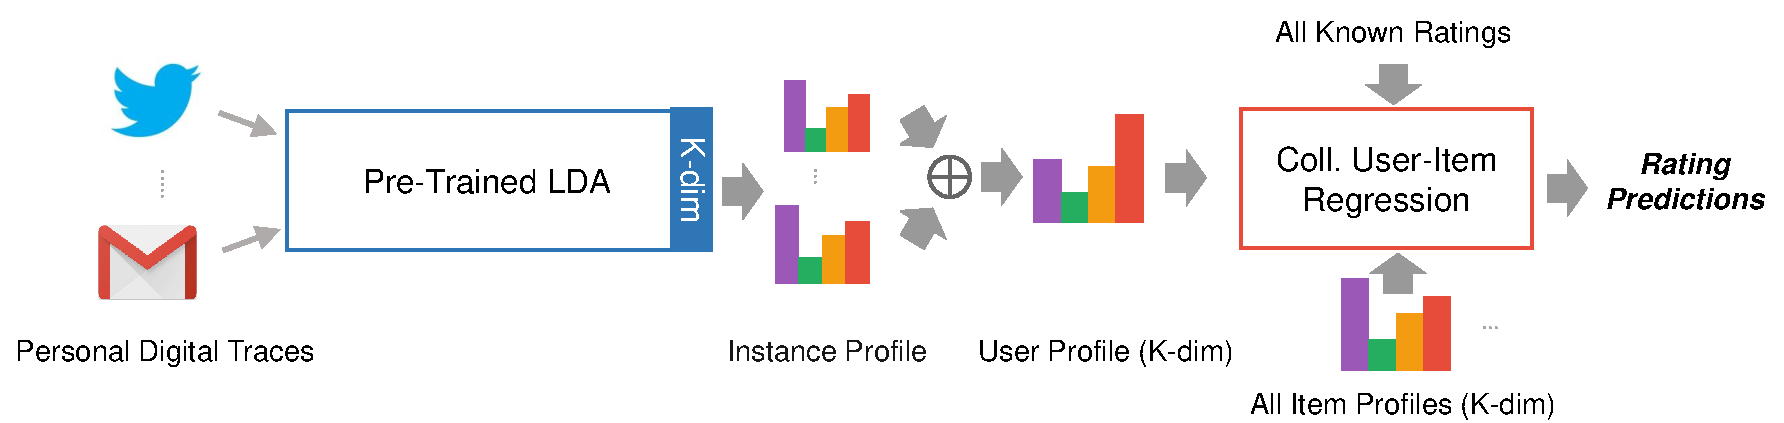
\includegraphics[width=.95\textwidth]{images/overview}
\caption{An overview of the proposed recommendation framework. For each user, a user profile is derived from the latent topical distributions in her digital traces learned via LDA. This profile is then used to fuel a novel collaborative filtering model that is able to incorporate user and item profiles as well as all the known ratings to generate rating prediction and recommendations.}
\label{fig:overview}
\end{figure*}

An overview of our recommendation framework is illustrated in Figure \ref{fig:overview} and described as follows: in the user profiling phase, for each user $i$, a user profile $\mathbf{u}_i$ is derived from her digital traces. We focus on text-based traces in this paper; a trace instance $t$, for example, can be an email thread or a set of relevant tweets that users authorize the system to fetch from their accounts. In the recommendation phase, the system recommends items based on the predicted rating the user $i$ would give to item $j$, denoted by $\hat{r}_{ij}$. The rating prediction is done by a generative model that incorporates the user profile $\mathbf{u}_i$, item profile $\mathbf{v}_j$, and all known ratings into the prediction process. In the following, we describe the key design decisions for each phase.

\subsection{User Profiling Phase}
In the user profiling phase, for each user $i$, we extract user profile $\mathbf{u}_i$ from her digital traces. The challenge here is: \textit{how to turn users' unstructured digital traces into features with predictive power for that users' preferences?} Recent work in social recommendation proposed a memory-based approach that \textit{memorizes} all the instances in a user's digital traces, in particular friends and likes on social media, and uses the preferences of other users who share the same instances to make recommendations \cite{Sedhain:2014:SCF}. This approach, however, is not feasible for many personal traces where co-occurrences of instances are rare. For example, two users rarely possess the same email thread or tweets.

In order to incorporate a wider range of personal traces, we propose a content-based approach. For each instance $t$ in a user's digital traces, we derive a latent vector $\mathbf{y}_t \in \mathbb{R}^K$ that projects instance $t$ to a latent $K$-dimensional space based on its content. Similarly, for each item $j$, we derive a latent vector $\mathbf{v}_j \in \mathbb{R}^K$ that projects the item $j$ to the same $K$-dimensional space based on item $j$'s content. In this way, the \textit{relevance} between instance $t$ and item $j$ can be estimated from their geometric features (e.g. distances) in this shared latent space. 

As digital traces and items we consider in this paper both consist of textual data, our system uses \textit{Latent Dirichlet Allocation} (LDA) to conduct unsupervised topic modeling to create a transformation function $f$ that transforms trace instances and items into their corresponding latent representations based on their topic distributions \cite{Blei:2003}. More specifically, we assume there are $K$ topics, where each of trace instances $t$ or item $j$ arises from a mixture of topics, and each topic has a word distribution $\beta_{k} \sim $ Dirichlet($\phi$) \footnote{We assume a general familiarity with LDA throughout the paper (see \cite{Blei:2012:PTM:2133806.2133826} for a review)}. For each trace instance $t$, we denote its content as $d_t$. The generative process of $d_t$ as follows:
\begin{enumerate}
\item Draw topic proportions $\mathbf{\theta}_t \sim $ Dirichlet($\alpha$)
\item For each word $n$,
    \begin{enumerate}
        \item Draw topic assignment $z_{tn} \sim $ Mult($\theta_m$)
        \item Draw word $w_{tn} \sim $ Mult($\beta_{z_{tn}}$)
    \end{enumerate}
\end{enumerate} This process shows how each word in $d_t$ is drawn from the topic distribution $\mathbf{\theta}_t$ specific to instance $t$. The concentration parameter $\alpha$ is set in a way that $0 < \alpha < 1$, and $\mathbf{\theta}_t$ will concentrate on only a few topics to encourage the words that occur in the same document to be assigned the same topic. 

We develop a paralleled Gibbs sampler to estimate the maximum a priori (MAP) of topic distribution $\mathbf{\theta}_t$ as in \cite{mccallum2002mallet}, and use $\theta_t$ as the latent representation of instance $t$ (i.e. $\mathbf{y}_t=\mathbf{\theta}_t$). The same procedure applies to items, where we assume each item is generated by the same generative process and share the same word distributions $\beta_{1:K}$ with trace instances. An item's latent representation, similarly is set to be its topic distribution $\mathbf{\theta}_j$ (i.e. $\mathbf{v}_j=\mathbf{\theta}_j$). 

Through LDA, we are able to estimate the latent relevancy between instance $t$ and item $j$ even if they do not share the same contents. Take Alice, for example--as a backend software engineer, she may write an email to her colleagues proposing a plan to migrate their web-backend to Ruby on Rails. Based on this email, the system would recommend Alice articles that contain backend-engineering-related contents such as a study on Node.js or MongoDB, or possibly articles about the life of full-stack engineers even though these articles do not share exact content with Alice's email. Also, since LDA is unsupervised, it can learn topics, such as web development, or even self-driving cars, without them being predefined. 

One drawback of LDA, however, is that it requires a large amount of text contents to learn robust word distributions $\beta_{1:K}$, and users' digital traces are normally not available in the training time. Therefore, in practice, we pre-train the model using the contents of all the item $j$ and use the pre-train model to infer the topics distributions in users' digital traces. This allows us to estimate $\mathbf{y}_t$ in an on-demand and real-time fashion without training the model from scratch. 

%The assumption we make here is that the users' digital traces share the same $K$ topics and word distributions $\beta_{1:K}$ with the pre-trained model. This assumption, while a practical one, is not without its drawbacks as we will discuss in Section X.

Finally, for each user $i$, her profile $\mathbf{u}_i$ is represented by aggregating the latent representations $\mathbf{y}_t$ of her trace instance $t$ as follows:
\begin{eqnarray}\label{eq:u_i}
\mathbf{u}_i = \frac{\sum_{t} w_{it}\mathbf{y}_t}{Z_i},
\end{eqnarray}where normalization constant $Z_i=\|\sum_{t} w_{it} \mathbf{y}_t\|_{1}$, and $w_{it}$ is the weighting assigned to each instance $t$. In this way, $\mathbf{u}_i$ characterizes the user's overall interests distribution over $K$ topics by a \textit{weighted bag of topics} representations. The $w_{it}$ is assigned based on various criteria. For example, we assign the instances users personally generated a heavier weight than the instances users passively received. For example, an email the user wrote is assigned a slightly higher weight than an email the user forwarded. 

\subsection{Recommendation Phase}
With the user profile $\mathbf{u}_i$ generated, we develop a recommendation algorithm that predicts the rating each user $i$ will give to each item $j$, denoted by $\hat{r}_{ij}$, and make recommendations accordingly. Our algorithm is a hybrid approach in the sense that it utilizes all the available data, including 1) known ratings, 2) item profile, and 3) user profile. These diverse data sources play important but different roles in generating high-quality recommendations. The objective information, including user profile and item profile\footnote{An item's profile is defined as its latent topic distributions inferred previously.}, generated in the previous phase, allows us to recommend items that are relevant to a user's interests; while the subjective information, including known ratings, allows us to estimate users' \textit{perceived quality} of an item. The perceived quality is defined as a consumer's opinion of a product's ability to fulfill his or her expectations \cite{jacoby1971price}, and is crucial in generating high-quality recommendations. For example, consider Alice, and a real article, \textit{io.js Week of March 6th Update}; judging from the content, this article is of high-relevancy to Alice's interests. However, a mundane software changes report like this is probably not going to be liked by Alice as it does not provide information or stories Alice would enjoy reading. It is hard to infer this perceived quality by objectively profiling content, in part because it is a perception and also because it is involved in the personal judgments from the user. On the other hand, what has more predictive power is the opinions of other people, in particular, the people who share a similar taste or interests with the targeted user \cite{Su:2009:SCF:1592474.1722966,}. Our model is designed to systematically combine these heterogeneous objective and subjective information and make recommendations that are not just relevant to users' interests, but also have high chance of satisfying their expectation.

Another issue our algorithm tries to solve is that a user's interests are not always consistent with what is shown in her profile. For example, while Alice has a variety of interests, she might only look for baby-care-related information on an e-magazine website for young parents, or she might be interested in some things that are entirely unseen from her digital traces. An ideal recommendation system should take this potential discrepancy into account and fine-tune the recommendations as soon as the user feedback is available. 

We propose a new \textit{collaborative user-item regression} model as a comprehensive solution to the above-mentioned issues. On top of item profile $\mathbf{v}_j$, and user profile $\mathbf{u}_i$, this model additionally includes \textit{latent user offset} $\mathbf{\eta}_i  \in \mathbb{R}^K$ and \textit{latent item offset} $\mathbf{\epsilon}_j  \in \mathbb{R}^K$, which are learned in a user-user collaborative fashion. More specifically, let $r_{ij}$ denote the known rating user $i$ gave to item $j$, and set $r_{ij}=1$ if the user $i$ upvoted item $j$, and $r_{ij}=0$ otherwise. The model assumes ratings $r_{ij}$ generated via the following generative process:

\begin{enumerate}
\item For each user $i$, draw user offset $\mathbf{\eta}_i \sim \mathcal{N}(0, \lambda_u^{-1}I_K)$
\item For each item $j$, draw item offset $\mathbf{\epsilon}_i \sim \mathcal{N}(0, \lambda_v^{-1}I_K)$
\item For each user-item pair $(i, j)$, draw the rating
\begin{eqnarray} \label{eq:r}
 r_{ij} \sim \mathcal{N}((\mathbf{u}_i+\mathbf{\eta}_i)^T(\mathbf{v}_j+\mathbf{\epsilon}_i), c_{ij}^{-1})
\end{eqnarray}
\end{enumerate}, where precision parameter $c_{ij}$ serves as a confidence parameter for rating $r_{ij}$, and is set larger if we trust the rating $r_{ij}$ more. Since the case $r_{ij}=0$ can be interpreted as either 1) the user did not like the item, or 2) the user was not aware of the item \cite{hu2008collaborative,wang2011collaborative}, we set $c_{ij}$ lower when $r_{ij}=0$ to account for this uncertainty, which is:

\begin{eqnarray}
c_{ij} = 
\begin{cases} 
a, & \mbox{if }  r_{ij} = 1 \\ 
b, & \mbox{if }  r_{ij} = 0 
\end{cases}
\end{eqnarray} where $a$ and $b$ are tuning parameter, and $a > b > 0$.

The key ingredient of this model lies in Eq. \ref{eq:r}. As $\mathbf{v}_j$ and $\mathbf{u}_i$ are fixed, Eq. \ref{eq:r} encourages the offset $\mathbf{\epsilon}_i$ and $\mathbf{\eta}_j$ to adjust for two different latent forces that are unseen in the objective profile information, but play important roles in generating the ratings as follows. The item offset $\mathbf{\epsilon}_j$ accounts for different groups of users' perceived quality of item $j$. Taking a real article \textit{The Difference Between Living in New York and San Francisco} for example \cite{articleSample}, while this article does not have content related to technology, many tech people enjoy this article as these are the two cities where many of them live or consider moving to. Therefore, the offset $\mathbf{\epsilon}_j$ tends to have a higher weight in the dimension corresponding to the tech-related topic to adjust for this group of people's perceived quality of this item. 

On the other hand, the user offset $\mathbf{\eta}_i$ accounts for the difference between a user's initial profile $\mathbf{u}_i$ and the interests she expresses in the stories she upvoted. For a new user who has not made any upvotes, her offset $\mathbf{\eta}_i$ is be a zero vector. However, once she starts to give ratings, $\mathbf{\eta}_i$ will be adjusted for the preferences (both negative or positive) that are not captured by her profile $\mathbf{u}_i$, and enable a much finer-tuned recommendation. Finally, $\lambda_v$ and $\lambda_u$ are the regularization parameters that determine the scale of the offsets. For example, if $\lambda_u$ is smaller, a larger scale of $\eta_i$ is allowed, and the recommendation will lean more towards the preferences expressed in user $i$'s ratings than towards her initial profile $\mathbf{u}_i$.

\subsection{Parameter learning}
Since directly computing the posterior distribution of $\mathbf{\epsilon}_j$ and $\mathbf{\eta}_i$ is intractable \cite{wang2011collaborative}, we develop an EM-algorithm \cite{dempster1977maximum} to estimate their maximum a posteriori probability (MAP):

The complete log likelihood of $\mathbf{\eta}_i$ , and $\mathbf{\epsilon}_j$ is: 

\begin{eqnarray}
\begin{split}
\mathbb{L} &= - \frac{\lambda_{u}}{2}\sum_{i}\mathbf{\eta}_i^{T}\mathbf{\eta}_i 
             - \frac{\lambda_{v}}{2}\sum_{j}\mathbf{\epsilon}_j^{T}\mathbf{\epsilon}_j \\
        &     - \sum_{i,j}\frac{c_{ij}}{2}(r_{ij}-(u_i+\eta_i)^T(v_j+\epsilon_j))
\end{split}
\end{eqnarray}
We optimize the log-lokelihood $\mathbb{L}$ by a coordinated ascent. Let $\hat{u_i}=u_i+\eta_i$, $\hat{v_j}=v_j+\epsilon_j$, and  $\hat{U}=\hat{u_i}^I_{i=1}$, $\hat{V}=\hat{v_j}^J_{j=1}$. We take the gradient of $\mathbb{L}$ with respect to $\hat{u}$ and $\hat{v}$, respectively, setting them to zero to derive the optimization functions:

\begin{eqnarray}\label{eq:gradient_u}
\hat{u}_i \leftarrow (\hat{V}C_i\hat{V}^T + \lambda_uI_K)^{-1}(\hat{V}C_iR_i + \lambda_uu_i)\\
\label{eq:gradient_v}
\hat{v}_j \leftarrow (\hat{U}C_j\hat{U}^T + \lambda_vI_K)^{-1}(\hat{U}C_jR_j + \lambda_vv_j)
\end{eqnarray} where $C_i$ is a diagonal matrix with $c_{ij}$ for $j=1 ..., J$ as its diagonal elements and $R_i = (r_{ij})^J_{j=1}$ for user $i$. $C_j$ and $R_j$ are defined in a similar way for item $j$. 

With this optimization function, in each iteration, we update all $\hat{u_i}$ with the latest estimation of $\hat{v_j}$, then update all $\hat{v_j}$ with the latest estimation of $\hat{u_i}$ alternatively. This estimation process stops when the log-likelihood $\mathbb{L}$ converges, and the MAP of $\mathbf{\eta}_i$ and $\mathbf{\epsilon}_j$ is derived by subtracting profile $\mathbf{u}_i$ and $\mathbf{v}_j$ from $\hat{u_i}$ and $\hat{v_j}$ respectively. While the complexity of each iteration is linear to the number of known ratings $r_{ij}$, which can be quite large, each iteration enjoys a high degree of parallelism as all the $\hat{u_i}$ and all the $\hat{v_j}$ can be estimated concurrently.

\subsection{Prediction and New Rating Fold-In Process}\label{sec:fold-in}
After offsets $\mathbf{\eta}_i$ and $\mathbf{\epsilon}_j$ are learned, we use our model to predict the unseen ratings $\hat{r}_{ij}$ as follow:

\begin{eqnarray}\label{eq:r_estimated}
\hat{r}_{ij} \approx (\mathbf{u}_i+\eta_i)^T(\mathbf{v}_j+\epsilon_j),
\end{eqnarray} where $\hat{r}_{ij}$ is the expectation of the rating given all the available information.

This prediction procedure is extremely efficient and allows us to make predictions for a large number of items in real-time as shown in Section XXX. More importantly, our model allows new ratings to be \textit{folded in} the model and update the user offset $\mathbf{\eta}_i$. The updated $\mathbf{\eta}_i$ is computed by deriving the $\hat{\mathbf{u}}_i$ again with the updated $C_i$ and $R_i$ in Eq. \ref{eq:gradient_u}. This process, however, incurs major overhead in computing $\hat{V}C_i\hat{V}^T$, which has time complexity $O(J)$ and is too slow for most practical systems that need to respond to users' actions immediately. We optimize the fold-in process based on the observation that 
\begin{eqnarray}
\hat{V}C_i\hat{V}^T = b\hat{V}\hat{V}^T + (a-b)\sum\limits_{j\in S(i)} \hat{v_j}\hat{v_j}^T,
\end{eqnarray}
where $S(i)$ is the set of items user $i$ has upvoted. The optimization is done by caching $b\hat{V}\hat{V}^T$, and only computing $(a-b)\sum_j\in upvotes(i) \hat{v_j}\hat{v_j}^T$ in the fold-in procedure. This optimization introduces $\frac{J+|S(i)|}{|S(i)|}$ times of speed-up, which is quite significant as $J \gg |S(i)|$ in most cases.

\subsection{Related Models}
The proposed model belongs to the line of research in \textit{probabilistic matrix factorization}, where a generative process for rating $r_{ij}$ is assumed \cite{mnih2007probabilistic,Salakhutdinov:2008:BPM:1390156.1390267,Ma:2008:SSR:1458082.1458205,wang2011collaborative}. In particular, our model is an extension to  Wang and Blei's \textit{collaborative topic regression} model (CTR) \cite{wang2011collaborative}, where they only consider the item offset $\mathbf{\epsilon}_j$, and do not have user profile $\mathbf{u}_i$ and user offset  $\mathbf{\eta}_i$. As shown in Section \ref{sec:rec_perf}, the inclusion of $\mathbf{u}_i$ and $\mathbf{\eta}_i$ introduces a significant improvement over the CTR model. Other flavors of user-profile-boosted probabilistic models  include \textit{Regression-based latent factor model} \cite{Agarwal:2009}, \textit{Factorization Machines} \cite{rendle2012factorization}, and \textit{Pairwise Preference Regression} \cite{Park:2009}. However, most of them were designed to utilize categorical demographic data, such as age and gender, rather than unstructured personal data streams we consider in this paper. Also, our topic-model-based approach is semantically-meaningful and has the advantage in better recommendation diagnosability and transparency \cite{wang2011collaborative,Herlocker:2000:ECF:358916.358995}.


\section{Offline Evaluation}
We conducted a large-scale offline experiment with a publicly-available, Twitter-Medium.com dataset. We collected 53,401 users' complete upvotes history on Medium.com and their public twitter data. In total, over 25,000 Medium.com stories, 2M upvotes, and 24M tweets were collected. In the user profiling phase, as suggested in \cite{Bhattacharya:2014:IUI:2645710.2645765}, rather than treat each tweet as one instance, we take a set of tweets from the same source as one instance in order to infer a more robust topic distribution $\mathbf{y}_t$. Each user's trace instances consists of one instance that is composed of all tweets made by her and multiple instances, each of which is composed of the tweets made by each of her followees, or public tweets that contains each hashtag she used \footnote{The users' tweets were fetched from Twitter's Timeline API while the hashtag tweets were fetched from the Search API}. 

%Figure X shows the distribution of 1) numbers of each user' upvotes, 2) number of upvotes each item recveived, and 3) number of instances in each user's trace. The first two distributions 

In the following, we first study the predictive power of our user profiling strategy, and evaluate the accuracy of the proposed recommendation algorithm in predicting upvotes, followed by an evaluation of the algorithm efficiency in generating recommendations and fine-tuning the user profile for a large-sized item set.

\subsection{User Profile Predictive Power}
\begin{figure}[!t]
\centering
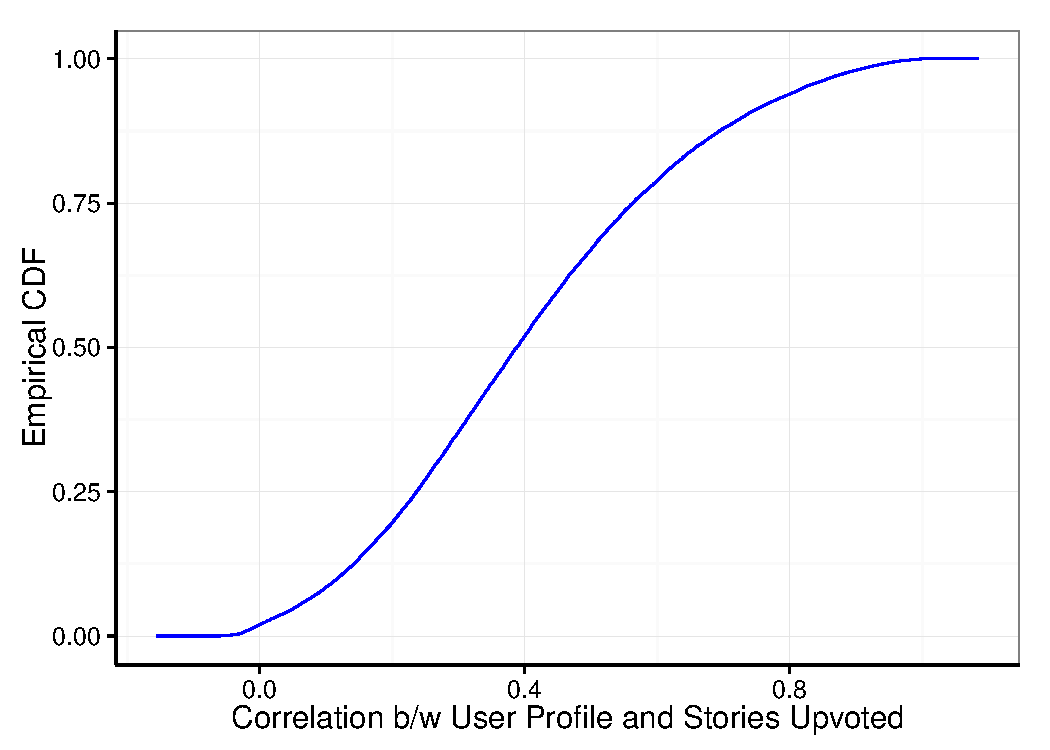
\includegraphics[width=2.5in]{images/profile-corr}
\caption{Empirical CDF of topical correlation between the user profile and the topic distributions of upvoted items. Among over 38,000 users, the average topical correlation is 0.41 where 70.1\% (51.5\%) of then has $p$-value $<$ 0.05 (0.01).}
\label{fig:corr}
\end{figure}
We study the predictive power of our user profiling strategy by evaluating the empirical topical correlation between a user's profile $\mathbf{u}_i$ and the aggregate profile of stories $j$ the user upvoted. This aggregate profile is denoted by $\mathbf{s}_i$ and is estimated in a similar way as in Eq. \ref{eq:u_i} but with instance profile $\mathbf{y}_t$ replaced by item profile $\mathbf{v}_j$ of each upvoted item. The topical correlation is defined as the Pearson's correlation coefficient between $\mathbf{u}_i$ and $\mathbf{s}_i$ as follows:

\begin{eqnarray}
 \rho(\mathbf{u}_i,\mathbf{s}_i) = \frac {(\mathbf{u}_i -  \bar{\mathbf{u}_i}) \cdot (\mathbf{s}_i - \bar{\mathbf{s}_i}) } { \left\| \mathbf{u}_i -  \bar{\mathbf{u}_i} \right\| \left\| \mathbf{s}_i - \bar{\mathbf{s}_i}\right\| } 
\end{eqnarray}

We compute the topical correlation for 38,345 users who have at least 10 upvotes and plot the empirical CDF in Figure \ref{fig:corr}. The average topical correlation among these users is 0.41 with $SD=0.22$. This correlation is statistically significant (i.e. $p$-value $<$ 0.05) for over 70\% of the users, which indicates that our user profiling strategy has strong predictive power for users' interests.

\subsection{Recommendation Performance}\label{sec:rec_perf}
\begin{figure*}[!t]
\centering
\subfigure[Recall@50]{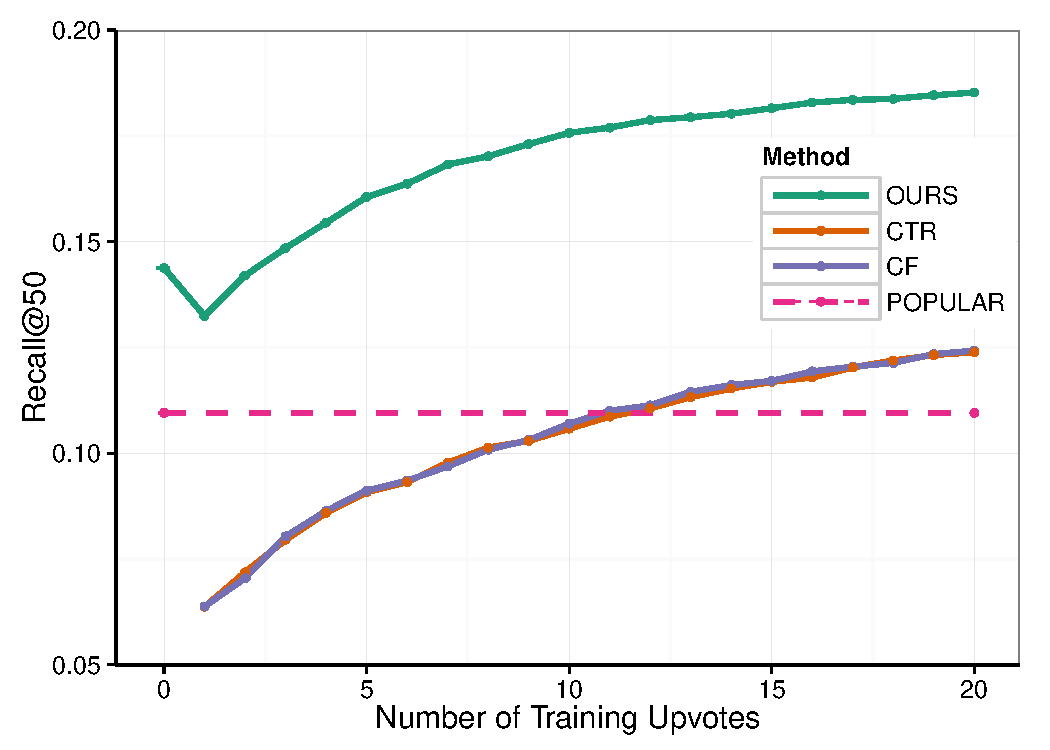
\includegraphics[width=.44\textwidth]{images/Recall_AT_50}}
\label{fig_first_case}
\quad\quad
\subfigure[nDCG@50]{{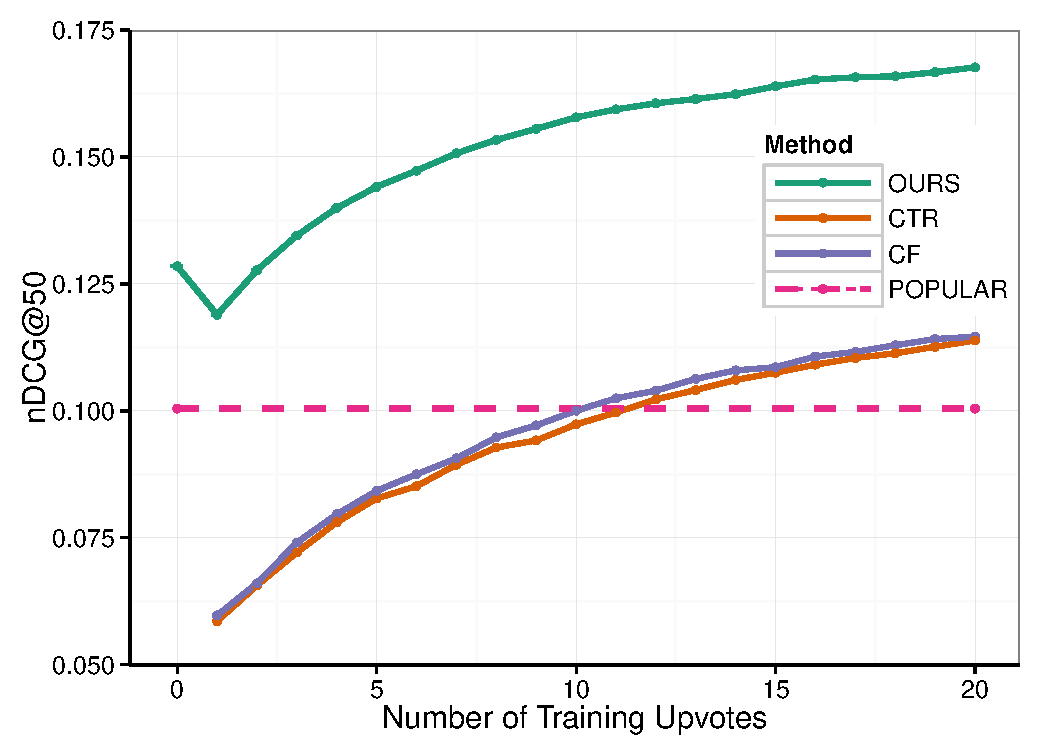
\includegraphics[width=.44\textwidth]{images/nDCG_AT_50}}
\label{fig_second_case}}
\caption{Average recommendation performances among 5,000 hold-out users when different numbers of upvotes from them are included in the model. Our approach significantly outperforms the second best approach in every scenario by at least 27.9\% up to 49.1\%, and achieve good accuracy even before a user made any upvote.}
\label{fig:rec_perf}
\end{figure*}


Next, we study the accuracy of our recommendation strategy by evaluating how accurate the algorithm can predict the stories a user actually upvoted.  We randomly chose 5,000 users to create a hold-out set whose entire upvote histories are excluded from the training of the model. We evaluate the recommendation accuracy for each hold-out user from the user-cold-start phase up to the point after they made 20 upvotes. We sequentially include the upvotes each hold-out users made \textbf{before} January 1st 2015 into the model, and make recommendations for only the stories published \textbf{after} January 1st 2015 to ensure each user's recommendations are made from the same pool of items. The upvotes from the hold-out users are fold-in in a chronological order as described in Section \ref{sec:fold-in} \footnote{The upvote time is approximated by the story publish time}. For each user and each scenario, we recommend top-50 stories based on the predicted ratings $\hat{r}_{ij}$, and compute the recall rate and normalized discounted cumulative gain (nDCG) of these 50 stories \cite{weimer2007maximum}. Note that we do not consider precision-related measurements, such as mAP, since we do not know a false-positive story did not get upvoted was because the user did not like it or simply because the user was not aware of it \cite{wang2011collaborative}. 

We compare our approach (denoted by \textbf{OURS}) with the following three competing algorithms: 
\begin{enumerate}
\item Most Popular First (\textbf{POPULAR}) that ranks the stories by number of upvotes they received. It is a common baseline for user-cold-start problem.

%\item Profile Recommender (\textbf{PROFILE}) that uses the cos-similarity between the user profile $\mathbf{u}_i$ and item profile $\mathbf{v}_j$ to rank items, and is a representative for pure profile-based approaches.

\item Probabilistic Matrix Factoring (\textbf{CF}) that makes recommendations based on $K$-dimensional latent factors. It is a representative for traditional user-user filtering approaches.

\item Collaborative Topic Regression (\textbf{CTR}) \cite{wang2011collaborative}, one of state-of-art document recommendation approaches, that considers both the item contents and user ratings. It is a representative for the existing hybrid algorithms. 
\end{enumerate}

We set $K=200$, $\lambda_u=10$, $\lambda_v=10$, $a=1$, and $b=0.01$, and plot the results in Figure \ref{fig:rec_perf}. As shown in Figure \ref{fig:rec_perf}, our approach significantly outperforms the second best approach by at least 27.9\% and up to 49.1\%  in different scenarios. More importantly, when a user has not made any upvote (i.e. in the user-cold-start phase), our approach is able to make recommendations that are more accurate than CF and CTR even after they includ 20 upvotes. That our algorithm keeps improving its accuracy with a larger number of included upvotes demonstrates the efficacy of our fine-tuning strategy \footnote{These trends also apply when top-100 stories are recommended.}. While the results indicate clear superiority of the proposed strategy, it also reveals a drawback of it when only few upvotes are available. Specifically, when users only make one upvote, the user offset $\mathbf{\eta}_i$ leans too much towards the profile of that item, and degrades the overall accuracy. This drawback can be addressed by putting a smoothing coefficient in front of $\mathbf{\eta}_i$ in Eq. \ref{eq:r_estimated} when the number of upvotes is small.


\subsection{Algorithm Efficiency}
Work in progress.......




\section{Future Work}

Work in progress.......

% An example of a floating figure using the graphicx package.
% Note that \label must occur AFTER (or within) \caption.
% For figures, \caption should occur after the \includegraphics.
% Note that IEEEtran v1.7 and later has special internal code that
% is designed to preserve the operation of \label within \caption
% even when the captionsoff option is in effect. However, because
% of issues like this, it may be the safest practice to put all your
% \label just after \caption rather than within \caption{}.
%
% Reminder: the "draftcls" or "draftclsnofoot", not "draft", class
% option should be used if it is desired that the figures are to be
% displayed while in draft mode.
%
%\begin{figure}[!t]
%\centering
%\includegraphics[width=2.5in]{myfigure}
% where an .eps filename suffix will be assumed under latex, 
% and a .pdf suffix will be assumed for pdflatex; or what has been declared
% via \DeclareGraphicsExtensions.
%\caption{Simulation Results}
%\label{fig_sim}
%\end{figure}

% Note that IEEE typically puts floats only at the top, even when this
% results in a large percentage of a column being occupied by floats.


% An example of a double column floating figure using two subfigures.
% (The subfig.sty package must be loaded for this to work.)
% The subfigure \label commands are set within each subfloat command, the
% \label for the overall figure must come after \caption.
% \hfil must be used as a separator to get equal spacing.
% The subfigure.sty package works much the same way, except \subfigure is
% used instead of \subfloat.
%
%\begin{figure*}[!t]
%\centerline{\subfloat[Case I]\includegraphics[width=2.5in]{subfigcase1}%
%\label{fig_first_case}}
%\hfil
%\subfloat[Case II]{\includegraphics[width=2.5in]{subfigcase2}%
%\label{fig_second_case}}}
%\caption{Simulation results}
%\label{fig_sim}
%\end{figure*}
%
% Note that often IEEE papers with subfigures do not employ subfigure
% captions (using the optional argument to \subfloat), but instead will
% reference/describe all of them (a), (b), etc., within the main caption.


% An example of a floating table. Note that, for IEEE style tables, the 
% \caption command should come BEFORE the table. Table text will default to
% \footnotesize as IEEE normally uses this smaller font for tables.
% The \label must come after \caption as always.
%
%\begin{table}[!t]
%% increase table row spacing, adjust to taste
%\renewcommand{\arraystretch}{1.3}
% if using array.sty, it might be a good idea to tweak the value of
% \extrarowheight as needed to properly center the text within the cells
%\caption{An Example of a Table}
%\label{table_example}
%\centering
%% Some packages, such as MDW tools, offer better commands for making tables
%% than the plain LaTeX2e tabular which is used here.
%\begin{tabular}{|c||c|}
%\hline
%One & Two\\
%\hline
%Three & Four\\
%\hline
%\end{tabular}
%\end{table}


% Note that IEEE does not put floats in the very first column - or typically
% anywhere on the first page for that matter. Also, in-text middle ("here")
% positioning is not used. Most IEEE journals/conferences use top floats
% exclusively. Note that, LaTeX2e, unlike IEEE journals/conferences, places
% footnotes above bottom floats. This can be corrected via the \fnbelowfloat
% command of the stfloats package.



\section{Conclusion}
The conclusion goes here.




% conference papers do not normally have an appendix


% use section* for acknowledgement
% \section*{Acknowledgment}






% trigger a \newpage just before the given reference
% number - used to balance the columns on the last page
% adjust value as needed - may need to be readjusted if
% the document is modified later
%\IEEEtriggeratref{8}
% The "triggered" command can be changed if desired:
%\IEEEtriggercmd{\enlargethispage{-5in}}

% references section

% can use a bibliography generated by BibTeX as a .bbl file
% BibTeX documentation can be easily obtained at:
% http://www.ctan.org/tex-archive/biblio/bibtex/contrib/doc/
% The IEEEtran BibTeX style support page is at:
% http://www.michaelshell.org/tex/ieeetran/bibtex/
\bibliographystyle{IEEEtran}
% argument is your BibTeX string definitions and bibliography database(s)
\bibliography{IEEEabrv,IEEEexample}
%
% <OR> manually copy in the resultant .bbl file
% set second argument of \begin to the number of references
% (used to reserve space for the reference number labels box)





% that's all folks
\end{document}


